% Options for packages loaded elsewhere
\PassOptionsToPackage{unicode}{hyperref}
\PassOptionsToPackage{hyphens}{url}
%
\documentclass[
  12pt,
]{article}
\usepackage{amsmath,amssymb}
\usepackage{lmodern}
\usepackage{iftex}
\ifPDFTeX
  \usepackage[T1]{fontenc}
  \usepackage[utf8]{inputenc}
  \usepackage{textcomp} % provide euro and other symbols
\else % if luatex or xetex
  \usepackage{unicode-math}
  \defaultfontfeatures{Scale=MatchLowercase}
  \defaultfontfeatures[\rmfamily]{Ligatures=TeX,Scale=1}
\fi
% Use upquote if available, for straight quotes in verbatim environments
\IfFileExists{upquote.sty}{\usepackage{upquote}}{}
\IfFileExists{microtype.sty}{% use microtype if available
  \usepackage[]{microtype}
  \UseMicrotypeSet[protrusion]{basicmath} % disable protrusion for tt fonts
}{}
\makeatletter
\@ifundefined{KOMAClassName}{% if non-KOMA class
  \IfFileExists{parskip.sty}{%
    \usepackage{parskip}
  }{% else
    \setlength{\parindent}{0pt}
    \setlength{\parskip}{6pt plus 2pt minus 1pt}}
}{% if KOMA class
  \KOMAoptions{parskip=half}}
\makeatother
\usepackage{xcolor}
\usepackage[margin=1in]{geometry}
\usepackage{color}
\usepackage{fancyvrb}
\newcommand{\VerbBar}{|}
\newcommand{\VERB}{\Verb[commandchars=\\\{\}]}
\DefineVerbatimEnvironment{Highlighting}{Verbatim}{commandchars=\\\{\}}
% Add ',fontsize=\small' for more characters per line
\usepackage{framed}
\definecolor{shadecolor}{RGB}{248,248,248}
\newenvironment{Shaded}{\begin{snugshade}}{\end{snugshade}}
\newcommand{\AlertTok}[1]{\textcolor[rgb]{0.94,0.16,0.16}{#1}}
\newcommand{\AnnotationTok}[1]{\textcolor[rgb]{0.56,0.35,0.01}{\textbf{\textit{#1}}}}
\newcommand{\AttributeTok}[1]{\textcolor[rgb]{0.77,0.63,0.00}{#1}}
\newcommand{\BaseNTok}[1]{\textcolor[rgb]{0.00,0.00,0.81}{#1}}
\newcommand{\BuiltInTok}[1]{#1}
\newcommand{\CharTok}[1]{\textcolor[rgb]{0.31,0.60,0.02}{#1}}
\newcommand{\CommentTok}[1]{\textcolor[rgb]{0.56,0.35,0.01}{\textit{#1}}}
\newcommand{\CommentVarTok}[1]{\textcolor[rgb]{0.56,0.35,0.01}{\textbf{\textit{#1}}}}
\newcommand{\ConstantTok}[1]{\textcolor[rgb]{0.00,0.00,0.00}{#1}}
\newcommand{\ControlFlowTok}[1]{\textcolor[rgb]{0.13,0.29,0.53}{\textbf{#1}}}
\newcommand{\DataTypeTok}[1]{\textcolor[rgb]{0.13,0.29,0.53}{#1}}
\newcommand{\DecValTok}[1]{\textcolor[rgb]{0.00,0.00,0.81}{#1}}
\newcommand{\DocumentationTok}[1]{\textcolor[rgb]{0.56,0.35,0.01}{\textbf{\textit{#1}}}}
\newcommand{\ErrorTok}[1]{\textcolor[rgb]{0.64,0.00,0.00}{\textbf{#1}}}
\newcommand{\ExtensionTok}[1]{#1}
\newcommand{\FloatTok}[1]{\textcolor[rgb]{0.00,0.00,0.81}{#1}}
\newcommand{\FunctionTok}[1]{\textcolor[rgb]{0.00,0.00,0.00}{#1}}
\newcommand{\ImportTok}[1]{#1}
\newcommand{\InformationTok}[1]{\textcolor[rgb]{0.56,0.35,0.01}{\textbf{\textit{#1}}}}
\newcommand{\KeywordTok}[1]{\textcolor[rgb]{0.13,0.29,0.53}{\textbf{#1}}}
\newcommand{\NormalTok}[1]{#1}
\newcommand{\OperatorTok}[1]{\textcolor[rgb]{0.81,0.36,0.00}{\textbf{#1}}}
\newcommand{\OtherTok}[1]{\textcolor[rgb]{0.56,0.35,0.01}{#1}}
\newcommand{\PreprocessorTok}[1]{\textcolor[rgb]{0.56,0.35,0.01}{\textit{#1}}}
\newcommand{\RegionMarkerTok}[1]{#1}
\newcommand{\SpecialCharTok}[1]{\textcolor[rgb]{0.00,0.00,0.00}{#1}}
\newcommand{\SpecialStringTok}[1]{\textcolor[rgb]{0.31,0.60,0.02}{#1}}
\newcommand{\StringTok}[1]{\textcolor[rgb]{0.31,0.60,0.02}{#1}}
\newcommand{\VariableTok}[1]{\textcolor[rgb]{0.00,0.00,0.00}{#1}}
\newcommand{\VerbatimStringTok}[1]{\textcolor[rgb]{0.31,0.60,0.02}{#1}}
\newcommand{\WarningTok}[1]{\textcolor[rgb]{0.56,0.35,0.01}{\textbf{\textit{#1}}}}
\usepackage{graphicx}
\makeatletter
\def\maxwidth{\ifdim\Gin@nat@width>\linewidth\linewidth\else\Gin@nat@width\fi}
\def\maxheight{\ifdim\Gin@nat@height>\textheight\textheight\else\Gin@nat@height\fi}
\makeatother
% Scale images if necessary, so that they will not overflow the page
% margins by default, and it is still possible to overwrite the defaults
% using explicit options in \includegraphics[width, height, ...]{}
\setkeys{Gin}{width=\maxwidth,height=\maxheight,keepaspectratio}
% Set default figure placement to htbp
\makeatletter
\def\fps@figure{htbp}
\makeatother
\setlength{\emergencystretch}{3em} % prevent overfull lines
\providecommand{\tightlist}{%
  \setlength{\itemsep}{0pt}\setlength{\parskip}{0pt}}
\setcounter{secnumdepth}{5}
\newlength{\cslhangindent}
\setlength{\cslhangindent}{1.5em}
\newlength{\csllabelwidth}
\setlength{\csllabelwidth}{3em}
\newlength{\cslentryspacingunit} % times entry-spacing
\setlength{\cslentryspacingunit}{\parskip}
\newenvironment{CSLReferences}[2] % #1 hanging-ident, #2 entry spacing
 {% don't indent paragraphs
  \setlength{\parindent}{0pt}
  % turn on hanging indent if param 1 is 1
  \ifodd #1
  \let\oldpar\par
  \def\par{\hangindent=\cslhangindent\oldpar}
  \fi
  % set entry spacing
  \setlength{\parskip}{#2\cslentryspacingunit}
 }%
 {}
\usepackage{calc}
\newcommand{\CSLBlock}[1]{#1\hfill\break}
\newcommand{\CSLLeftMargin}[1]{\parbox[t]{\csllabelwidth}{#1}}
\newcommand{\CSLRightInline}[1]{\parbox[t]{\linewidth - \csllabelwidth}{#1}\break}
\newcommand{\CSLIndent}[1]{\hspace{\cslhangindent}#1}
\ifLuaTeX
\usepackage[bidi=basic]{babel}
\else
\usepackage[bidi=default]{babel}
\fi
\babelprovide[main,import]{spanish}
% get rid of language-specific shorthands (see #6817):
\let\LanguageShortHands\languageshorthands
\def\languageshorthands#1{}
\usepackage{dcolumn}
\usepackage{rotating}
\usepackage{xcolor}
\usepackage[bottom]{footmisc}
\usepackage{setspace}
\usepackage{multirow}
\usepackage{footnote}
\usepackage{caption}
\usepackage{subcaption}
\usepackage[font=small,labelfont=it,margin=\parindent,tableposition=top]{caption}
\usepackage{booktabs}
\usepackage{longtable}
\usepackage{array}
\usepackage{multirow}
\usepackage{wrapfig}
\usepackage{float}
\usepackage{colortbl}
\usepackage{pdflscape}
\usepackage{tabu}
\usepackage{threeparttable}
\usepackage{threeparttablex}
\usepackage[normalem]{ulem}
\usepackage{makecell}
\usepackage{xcolor}
\ifLuaTeX
  \usepackage{selnolig}  % disable illegal ligatures
\fi
\IfFileExists{bookmark.sty}{\usepackage{bookmark}}{\usepackage{hyperref}}
\IfFileExists{xurl.sty}{\usepackage{xurl}}{} % add URL line breaks if available
\urlstyle{same} % disable monospaced font for URLs
\hypersetup{
  pdflang={es-CO},
  hidelinks,
  pdfcreator={LaTeX via pandoc}}

\author{}
\date{\vspace{-2.5em}}

\begin{document}

\newpage
\begin{spacing}{0.9} 
\tableofcontents
\end{spacing}

\newpage

\begin{spacing}{0.9} 
\listoftables
\end{spacing}

\newpage
\listoffigures
\newpage
\normalsize

\hypertarget{introducciuxf3n}{%
\section{Introducción}\label{introducciuxf3n}}

\hypertarget{literatura-sobre-emotividad-y-polarizaciuxf3n}{%
\section{Literatura sobre emotividad y
polarización}\label{literatura-sobre-emotividad-y-polarizaciuxf3n}}

\hypertarget{fuentes-de-informaciuxf3n-y-preprocesamiento}{%
\section{Fuentes de información y
preprocesamiento}\label{fuentes-de-informaciuxf3n-y-preprocesamiento}}

Esta sección describe las principales características del dataset
utilizado y los procedimientos realizados durante el pre procesamiento
de la información. El dataset construido proviene de tres fuentes de
información: 1) textos parlamentarios emitidos desde 1965 a 2022; 2)
biografías parlamentarias y 3) votaciones dentro de la cámara de
diputados desde 2002 a 2022.

\hypertarget{textos-parlamentarios-biblioteca-del-congreso-nacional}{%
\subsection{Textos parlamentarios biblioteca del congreso
nacional}\label{textos-parlamentarios-biblioteca-del-congreso-nacional}}

Los textos parlamentarios corresponden a todas las transcripciones de
intervenciones parlamentarias realizadas en ambas cámaras desde el año
1965 hasta 2022. Debido a que no existe un set de datos ordenados de los
discursos parlamentarios, disponible para su descarga, la información
fue obtenida del sitio web de la Biblioteca del Congreso Nacional por
medio de técnicas de \emph{webscraping}
\footnote{En concreto, se desarrolló un código en R y por medio de una tecnología llamada Selenium se simuló un usuario que navegó a través de todos los discursos parlamentarios durante varias horas.}.
De esta manera, fueron obtenidas las transcripciones íntegras, junto a
algunos metadatos disponibles, como el título de la intervención, fecha
y autores de la misma.

La recolección de información tuvo como resultado un total de 579.663
intervenciones parlamentarias (tabla \ref{tab:tabla_pre_post_filtro}),
tanto individuales como grupales. Luego de una edición y selección de
intervenciones relevantes, el dataset final quedó conformado por 209.830
textos. Existen dos motivos que explican la reducción en la cantidad de
registros. En primer lugar, se seleccionaron solo aquellas
intervenciones en las que participa un solo parlamentario, de modo de
asociar claramente un discurso a una persona. El segundo motivo, guarda
relación con la remoción de ciertas categorías de intervenciones
parlamentarias que no son de interés para el presente estudio. Existen
52 categorías de participaciones parlamentarias, muchas de las cuales
corresponden a asuntos administrativos o tienen un lenguaje con un
fuerte sesgo técnico-jurídico. Dichas intervenciones fueron removidas,
puesto que no están asociados al objetivo de este trabajo
\footnote{Para más detalle sobre las categorías de participaciones parlamentarias ver Anexo}

\begin{table}[H]

\caption{\label{tab:tabla_pre_post_filtro}Total de intervenciones parlamentarias}
\centering
\begin{tabular}[t]{ll}
\toprule
filtro & cantidad de filas\\
\midrule
datos brutos & 579.663\\
datos filtrados & 209.830\\
\bottomrule
\end{tabular}
\end{table}

Tal como muestra la figura \ref{n_year}, existe una ventana de 17 años
en la que no se cuenta con información debido al cierre del Congreso
Nacional durante la dictadura
\footnote{No se muestran los datos de 2022 en el gráfico debido al bajo número de intervenciones existen en el momento de la recolección de información. Esta fue realizada durante marzo de 2022, de modo que a dicha fecha solo se registra una pequeña fracción de las intervenciones que usualmente se llevan a cabo durante un año legislativo}.

\begin{figure}[H]
\centering
\large
\caption{Número de intervenciones parlamentarias por año}
\label{n_year}
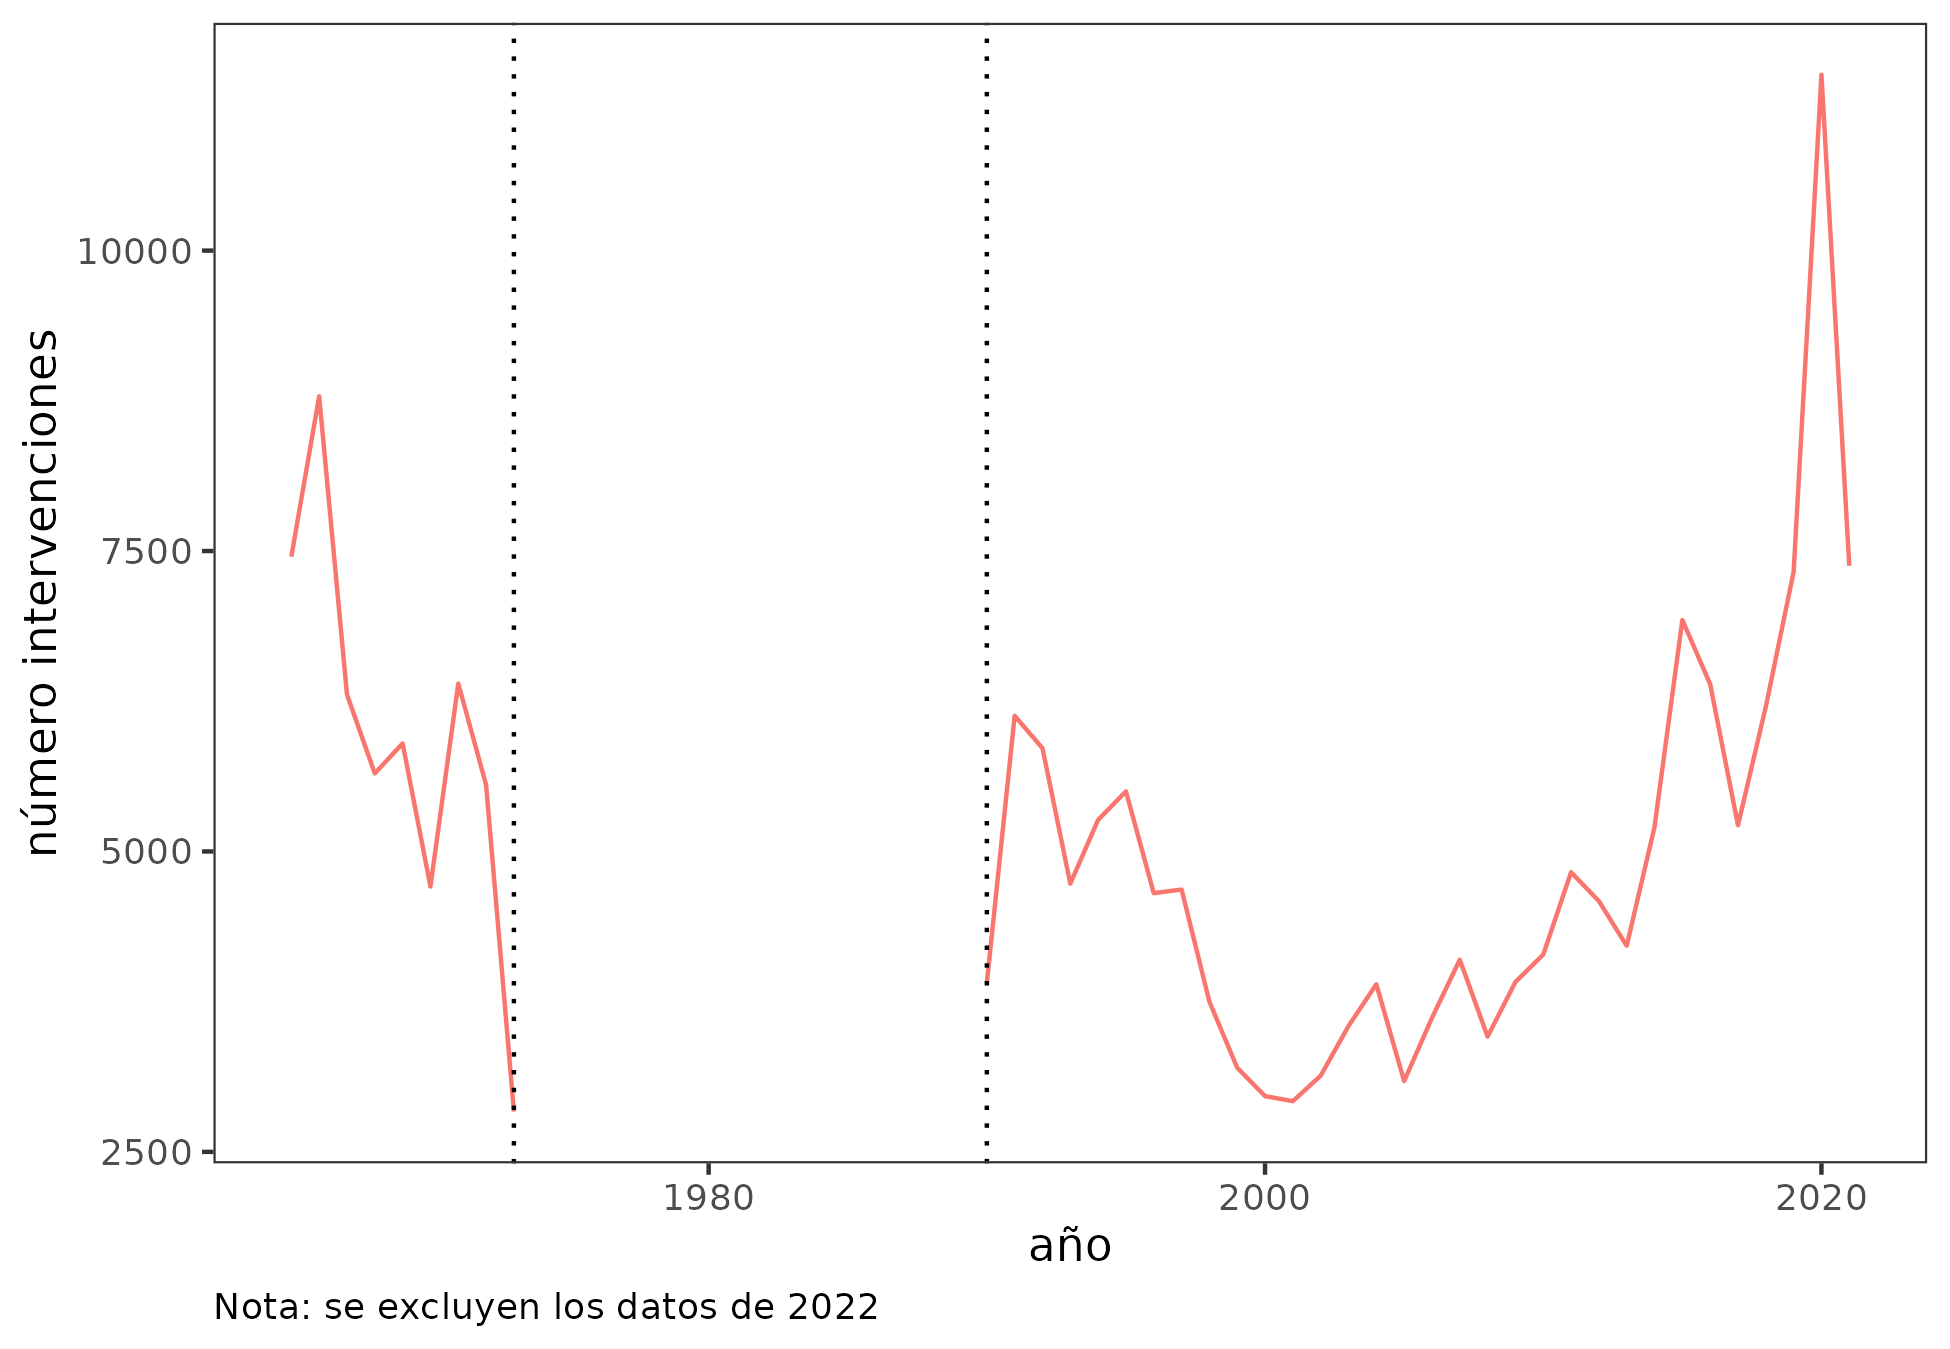
\includegraphics[width = 0.5 \textwidth]{cuadros_tesis/plot_n_year.png}
\normalsize
\end{figure}

Con el objeto de convertir los discursos parlamentarios en información
estadísticamente relevante, fue necesario llevar a cabo un
preprocesamiento de los datos. En primer lugar, se convirtieron todos
los textos en minúscula, lo cual facilita una serie de tareas del
procesamiento y reduce el número de palabras únicas. En segundo lugar,
se removieron algunos extractos de los textos poco informativos, como
los vocativos u otros encabezados similares
\footnote{Una gran cantidad de discursos comienza con el vocativo *señor presidente* o *señora presidenta*. Otro caso muy común ocurre cuando el presidente o presidenta de la cámara entrega la palabra, en cuyo caso suele utilizarse la fórmula *el/la diputado/a [nombre] tiene la palabra*}.

En tercer lugar, se dividieron los discursos en párrafos
\footnote{El separador utilizado fue el interlineado}, los cuales
constituyen la unidad de análisis que da lugar a los resultados de este
trabajo. Una vez separados en párrafos, los textos fueron
\emph{tokenizados} en palabras. Esto significa que cada intervención fue
dividida en párrafos y, a su vez, cada párrafo fue dividido en palabras,
las cuales corresponden a la unidad más desagregada posible.

En cuarto lugar, se removieron los signos de puntuación y las palabras
que en la terminología de NLP se denominan \emph{stopwords}. Estas
palabras se caracterizan por ser muy comunes, pues al corresponder a una
parte estructural de los idiomas, se utilizan en prácticamente todos los
contextos, por ende, para muchas tareas de clasificación de textos no
aportan información relevante. Por lo general, las librerías utilizadas
para NLP contienen listados de \emph{stopwords}, que típicamente
contienen conjunciones, preposiciones, algunos adverbios y otras
partículas.

Finalmente, se seleccionan los sustantivos, adjetivos y verbos mediante
un modelo de
\emph{spacy}\footnote{Spacy es una librería de Python ampliamente utilizada para facilitar tareas relacionadas con el procesamiento de lenguaje natural. Spacy contiene modelos para hacer POS, *name entity recognition*, mapeo de palabras a vectores, entre otras herramientas}
entrenado para hacer POS (\emph{Part of speech}). Mediante esta
operación se busca retener aquellas palabras que aportan más significado
al contenido de los discursos parlamentarios, lo cual además disminuye
el tiempo de computación, ya que se elimina una parte importante de las
palabras del corpus.

El cuadro \ref{tab:ejemplo_preprocesamiento} muestra un ejemplo de la
situación inicial y final de un extracto de una de las intervenciones
parlamentarias. Es posible observar lo siguiente: 1) el texto final está
en minúscula, 2) no existen signos de puntuación, 3) varias palabras han
sido removidas y 4) el párrafo original está contenido en una lista de
palabras.

\begin{table}[H]

\caption{\label{tab:ejemplo_preprocesamiento}Ejemplo de preprocesamiento}
\centering
\begin{tabular}[t]{>{\raggedright\arraybackslash}p{15em}>{\raggedright\arraybackslash}p{15em}}
\toprule
original & final\\
\midrule
\em{\textbf{Lo destaco, porque queremos trabajar en los proyectos de los parlamentarios. Hemos visto lo que se busca con este proyecto, el ministro de Hacienda ya había anticipado que queremos aliviar  a las familias en materia crediticia y compartimos el espíritu de lo que se quiere. Y eso es justamente lo que explica  que queramos trabajar sobre los diversos proyectos de ley que ustedes han empujado y han sacado adelante.}} & \em{\textbf{{}['destaco', 'queremos', 'trabajar', 'proyectos', 'parlamentarios', 'visto', 'busca', 'proyecto', 'ministro',  'anticipado', 'queremos', 'aliviar', 'familias', 'materia', 'crediticia', 'compartimos', 'espíritu',  'quiere', 'explica', 'queramos', 'trabajar', 'proyectos', 'ley', 'empujado', 'sacado']}}\\
\bottomrule
\end{tabular}
\end{table}

Para tener una idea general de las características del dataset, el
cuadro \ref{tab:descripcion_dataset} muestra algunos estadísticos de
resumen. Las 209.830 intervenciones, al ser separadas en unidades más
pequeñas, dan lugar a un total de 2.649.588 de párrafos.

\begin{table}[H]

\caption{\label{tab:descripcion_dataset}Estadísticos de resumen}
\centering
\begin{tabular}[t]{lllll}
\toprule
total intervenciones & total párrafos & total palabras & párrafos/intervención & palabras/intervención\\
\midrule
209.830 & 2.649.588 & 49.065.194 & 12,63 & 233,83\\
\bottomrule
\end{tabular}
\end{table}

Respecto a los párrafos (unidad de análisis), el cuadro
\ref{tab:descripcion_parrafos} y la figura
\ref{plot_descripcion_parrafos} muestran que el número promedio de
palabras es aproximadamente 19 y que, en general, los textos no son
demasiado extensos, ya que el 50\% tiene 15 palabras o menos y el 90\%
tiene 39 palabras o menos. El hecho de utilizar una unidad de análisis
más desagregada que la intervención, hace más sencilla la identificación
de características distintivas en el texto, las cuales cuales tienden a
oscurecerse al trabajar con los textos completos, cuya extensión
promedio es de 233 palabras.

\begin{table}[H]

\caption{\label{tab:descripcion_parrafos}Estadísticos de resumen de los párrafos}
\centering
\begin{tabular}[t]{rrrrr}
\toprule
media & mediana & mínimo & máximo & p90\\
\midrule
18.52 & 15 & 1 & 790 & 39\\
\bottomrule
\end{tabular}
\end{table}

\begin{figure}[H]
\centering
\large
\caption{Histograma del número de palabras por párrafo}
\label{plot_descripcion_parrafos}
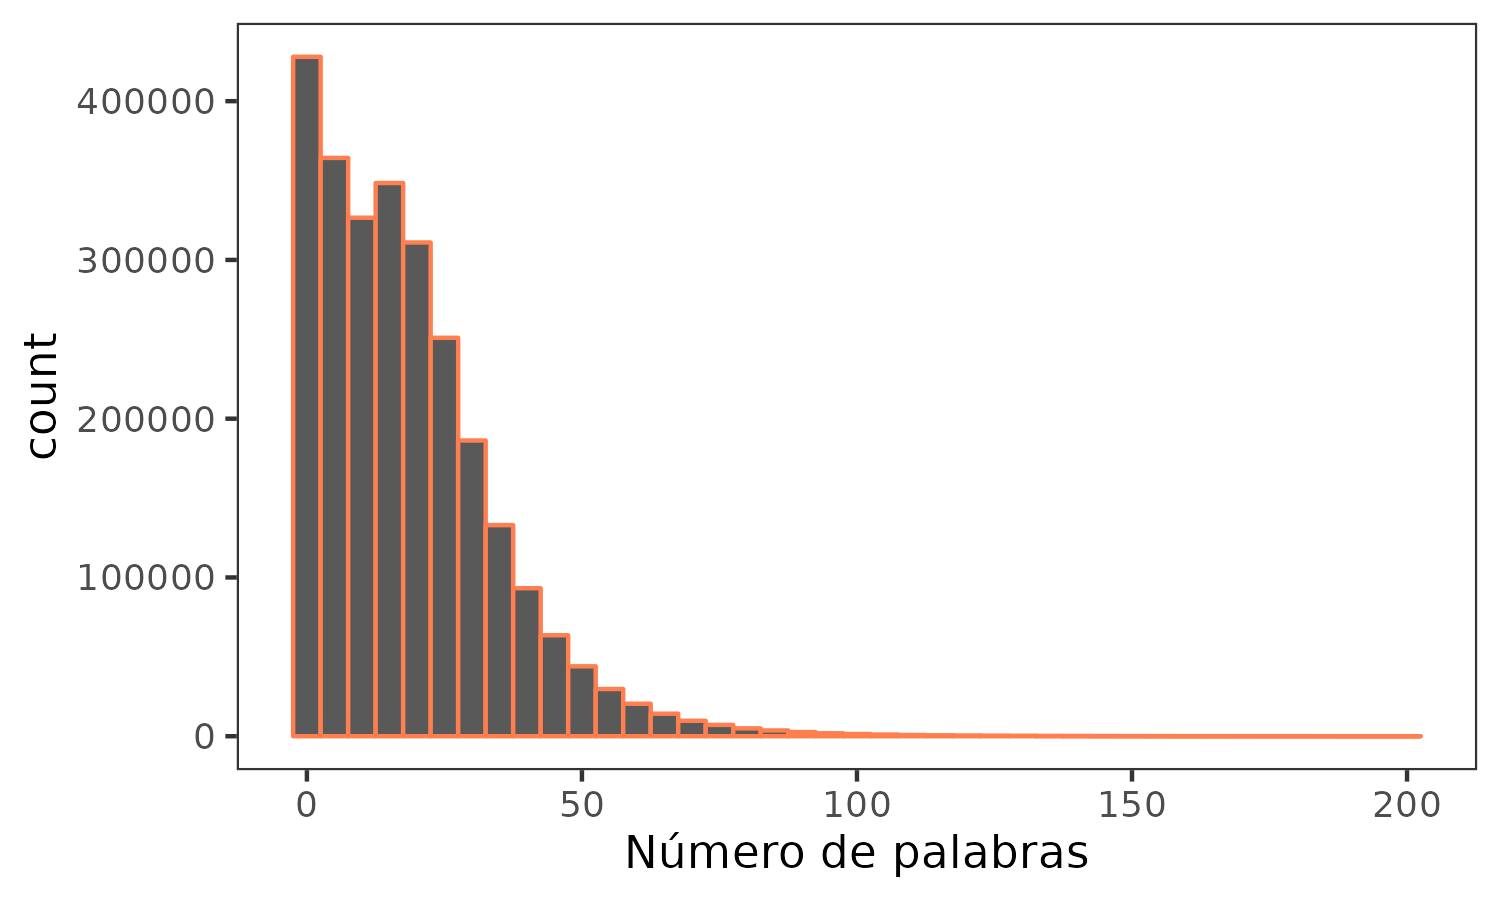
\includegraphics[width = 0.5 \textwidth]{cuadros_tesis/plot_hist_descripcion_parrafos.png}
\normalsize
\end{figure}

\hypertarget{biografuxedas-parlamentarias-biblioteca-del-congreso-nacional}{%
\subsection{Biografías parlamentarias biblioteca del congreso
nacional}\label{biografuxedas-parlamentarias-biblioteca-del-congreso-nacional}}

\hypertarget{votaciones-de-diputados}{%
\subsection{Votaciones de diputados}\label{votaciones-de-diputados}}

Para obtener la votación de los parlamentarios se recurrió a una API
dispuesta por la Cámara de Diputados, mediante la cual es posible
extraer todas las votaciones emitidas en la cámara baja desde 2002 en
adelante.

\hypertarget{metodologuxeda}{%
\section{Metodología}\label{metodologuxeda}}

Esta sección describe los principales aspectos metodológicos que se
encuentran a la base de los datos presentados en el apartado resultados.
Se entregan las principales características del diccionario utilizado,
la metodología de \emph{word embeddings} y cómo es que esta es utilizada
para ubicar cada texto en la polaridad cognitiva-afectiva.

\hypertarget{word-embeddings}{%
\subsection{\texorpdfstring{Word embeddings
\label{word_emb}}{Word embeddings }}\label{word-embeddings}}

El procesamiento de texto requiere llevar a cabo algún procedimiento
para convertir el lenguaje en una representación numérica que sea
legible para un algoritmo. Cualquier procedimiento que permita convertir
palabras en números se denomina \emph{word embeddings} (Skansi 2018).

Dentro de las estrategias para construir vectores de palabras, una de
las más utilizadas es el modelo \emph{Word2vec}, cuya idea fundamental
es que el significado de una palabra depende del contexto en el que esta
se encuentre. Siguiendo dicha noción, para aprender vectores de
palabras, se entrena una red neuronal utilizando grandes volúmenes de
texto, lo cual se puede llevar a cabo mediante dos estrategias
alternativas: CBOW (\emph{Continues Bag of Words}) o \emph{skip-gram}
(Charu C. 2018). En el modelo CBOW se entrena una red neuronal para que
prediga una palabra a partir de su contexto. Al contrario, en el enfoque
\emph{skip-gram} se utiliza una palabra para predecir el contexto.

Si se define que el contexto corresponde a dos palabras, en CBOW
utilizaremos las dos palabras anteriores y las dos posteriores para
predecir una palabra central. A la inversa, bajo la estrategia
\emph{skip-gram} se utiliza como entrada la palabra central, para
predecir las dos anteriores y dos posteriores.

En términos de arquitectura, los modelos están conformados por una capa
de entrada, una capa oculta y una capa de salida. La capa oculta
determina la cantidad de dimensiones que tendrán los vectores de
palabras. De este modo, si la capa escondida contiene 100 neuronas, el
número de dimensiones para representar cada palabra será 100. Cabe
señalar que tanto la capa de entrada como la de salida tienen el mismo
número de dimensiones, correspondiente a la cantidad de palabras
distintas en el corpus utilizado para llevar a cabo el entrenamiento.

Los modelos descritos no se diferencian en lo fundamental de los
autocodificadores (\emph{autoencoders}). Se busca llevar a cabo un
aprendizaje no supervisado (Skansi 2018), lo cual es posible gracias a
la disponibilidad de grandes volúmenes de texto y a la posibilidad de
procesar la información mediante una tarjeta gráfica. Ahora bien, debido
a que el proceso de entrenamiento por lo general es costoso, es
frecuente utilizar modelos desarrollados por personas u organizaciones
que cuentan con \emph{hardware} adecuado para este tipo de tareas.

En el marco de este trabajo se utilizaron los vectores entrenados por
(Perez y Cañete 2019) del Departamento de Ciencias de la Computación de
la Universidad de Chile. Los autores utilizan un algoritmo llamado
\emph{FastText} (Bojanowski et~al. 2016) sobre un corpus en español
llamado \emph{Spanish Unannotated Corpora} (SUC)
\footnote{Corpus construido a partir de una gran cantidad de fuentes. El dataset está conformado por 300 millones de líneas. Para mayores detalles sobre el dataset, ver https://github.com/josecannete/spanish-corpora}.
\emph{FastText} recoge la idea de que es posible capturar el significado
de las palabras a partir de sus contextos, sin embargo, se diferencia de
\emph{Word2Vec} en el hecho de que el texto no es dividido en palabras,
sino en conjuntos de caracteres más pequeños. El significado se
construye en este caso a partir de los caracteres que componen las
palabras. Ello hace posible, entre otras cosas, obtener vectores para
cualquier palabra, independiente de que estas hayan estado o no
presentes en el corpus de entrenamiento.

Pérez y Cañete (2019) ponen a disposición varios modelos, cuya
diferencia principal dice relación con el número de dimensiones que
tienen los vectores. El más pequeño está conformado por vectores de 10
dimensiones, mientras que el más grande, por vectores de 300
dimensiones. Con el objeto de acelerar el procesamiento de los datos
este trabajo utilizó el modelo de 100 dimensiones.

Los vectores de palabras construidos mediante \emph{FastText} y
\emph{Word2Vec} han demostrado ser capaces de capturar el significado de
las palabras. Así, palabras que aparecen en contextos similares, estarán
cerca en el espacio proyectado, lo cual implica que es posible llevar a
cabo operaciones algebraicas y agrupar palabras según la dirección en la
que apunten los vectores. Por ejemplo, si buscamos los vectores más
cercanos a \emph{rojo} (utilizando similitud coseno u otra medida de
distancia), se observa que el resultado corresponde a otros colores.

\begin{Shaded}
\begin{Highlighting}[]
\NormalTok{colores }\OperatorTok{=}\NormalTok{  wordvectors.most\_similar(positive}\OperatorTok{=}\NormalTok{[}\StringTok{\textquotesingle{}rojo\textquotesingle{}}\NormalTok{],  topn }\OperatorTok{=} \DecValTok{5}\NormalTok{)}
\end{Highlighting}
\end{Shaded}

\begin{table}[H]

\caption{\label{tab:tabla_colores}Palabras más cercanas a rojo}
\centering
\begin{tabular}[t]{lr}
\toprule
palabra & similitud\\
\midrule
amarillo & 0.906\\
azul & 0.903\\
blanco & 0.866\\
negro & 0.853\\
anaranjado & 0.843\\
\bottomrule
\end{tabular}
\end{table}

La idea de que las palabras cercanas tienen un correlato en el espacio
se puede expresar de manera gráfica mediante un ejercicio de reducción
de dimensionalidad. Dado que las palabras han sido convertidas en
vectores, es posible llevar a cabo procedimientos de reducción de
dimensionalidad. La figura \ref{plot_pca_ejemplo} corresponde a las dos
primeras componentes de un Análisis de Componentes Principales (PCA). Se
puede observar que al proyectar los vectores en este nuevo espacio de
dos dimensiones las posiciones de las palabras generan agrupaciones
conceptuales. De hecho, podemos observar tres grupos: animales, colores
y comidas.

\begin{figure}[H]
\centering
\large
\caption{Agrupación de palabras en un espacio bidimensional}
\label{plot_pca_ejemplo}
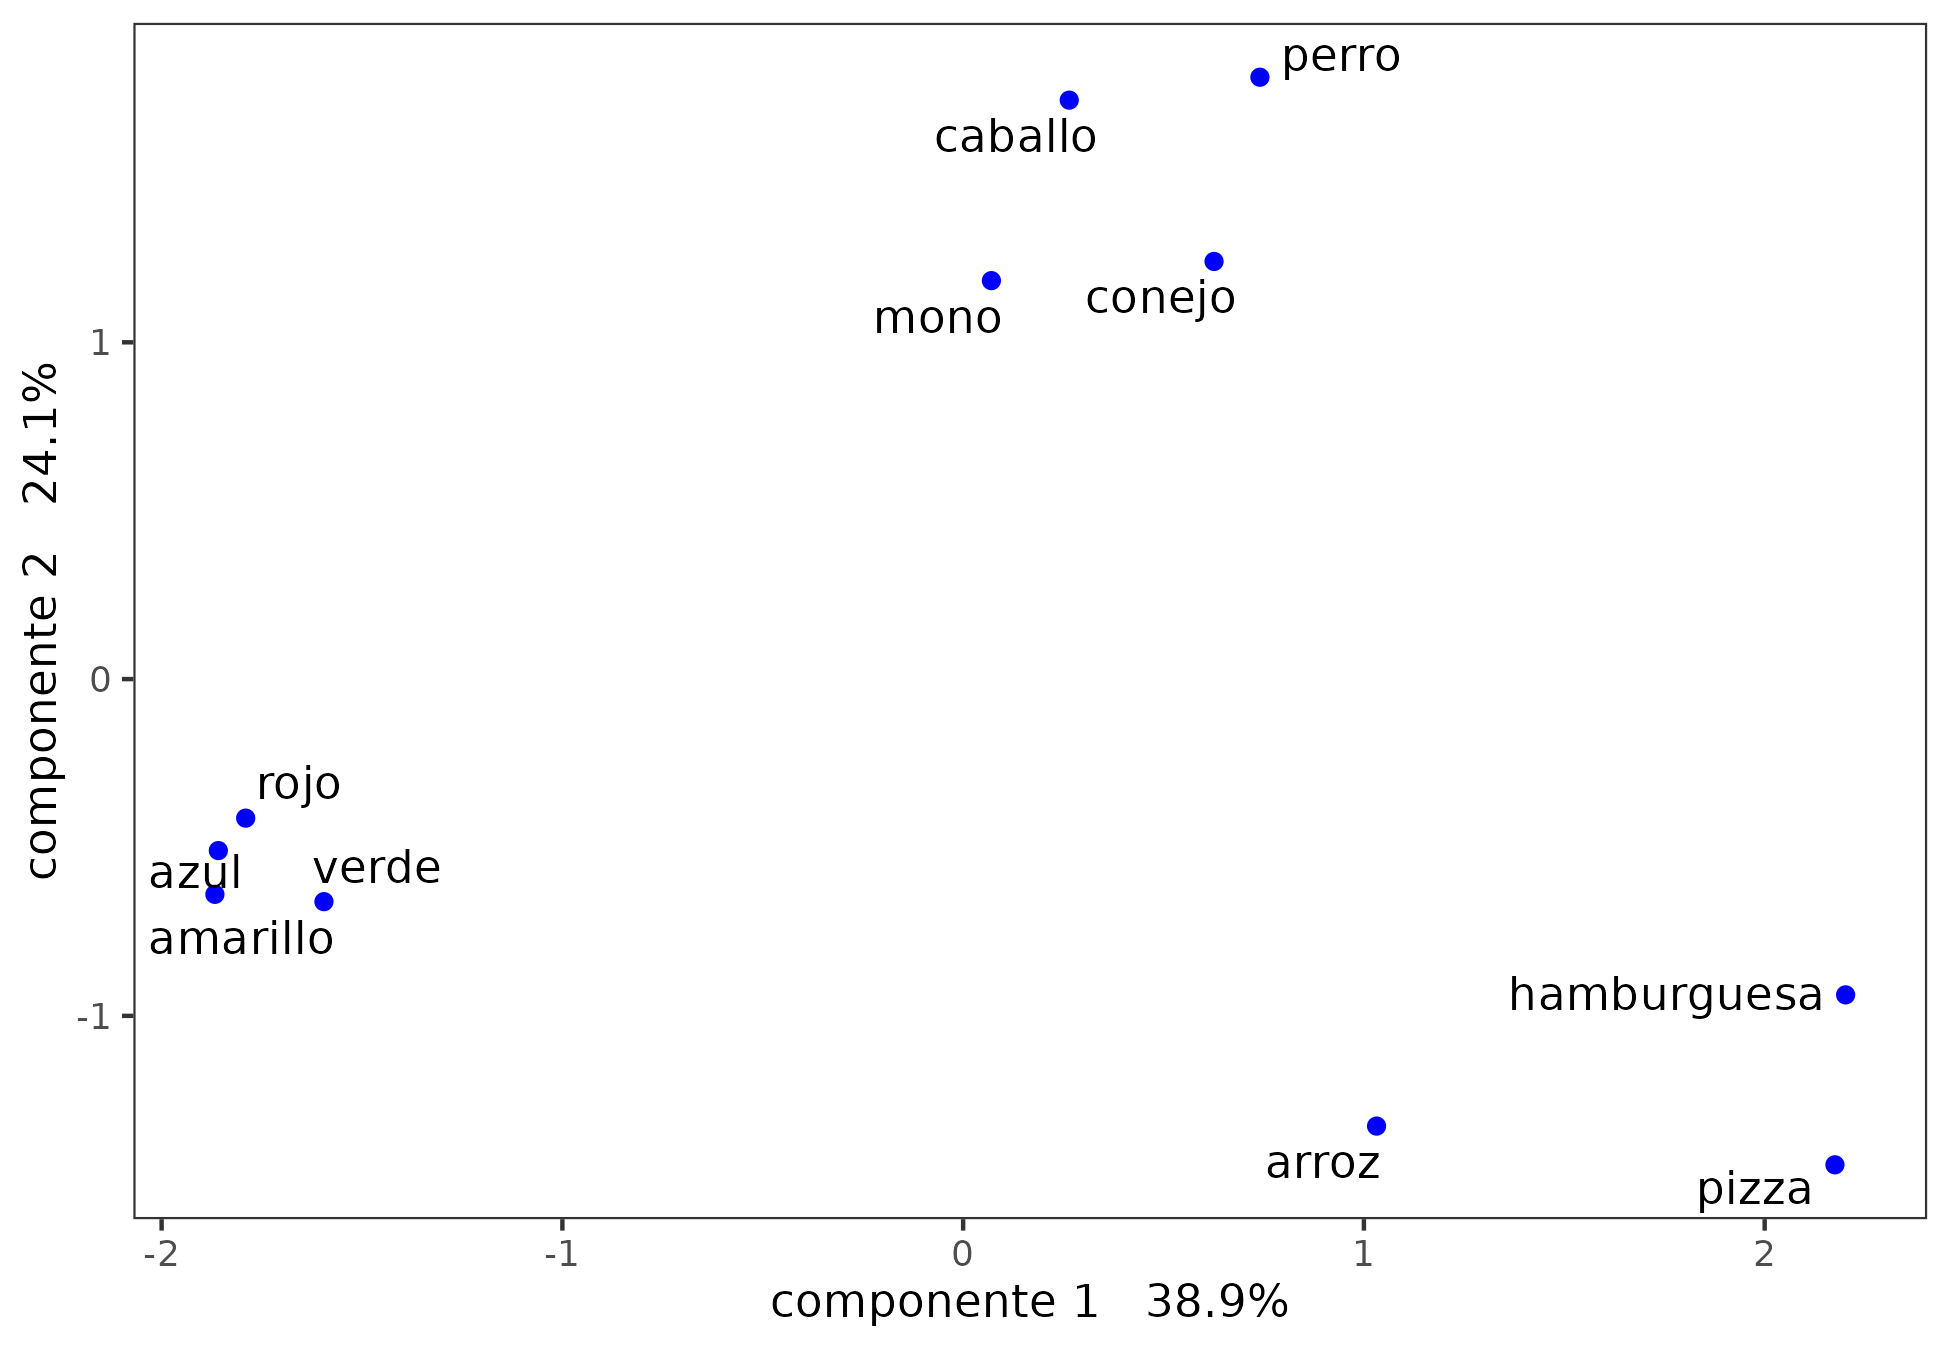
\includegraphics[width = 0.5 \textwidth]{cuadros_tesis/plot_pca.png}
\normalsize
\end{figure}

Los vectores también permiten construir analogías del tipo \(a\) es a
\(b\) como \(x\) es a \(y\) y establecer operaciones como la siguiente:

\[reina \approx rey - hombre + mujer\]

Mediante alguna medida de distancia (usualmente, similitud coseno) se
busca el vector más cercano a \(rey\) y a \(mujer\) y que, al mismo
tiempo, se aleje del vector \(hombre\). La tabla
\ref{tab:ejemplo_analogia} muestra que el vector más parecido,
efectivamente, corresponde a \emph{reina}, seguido por \emph{princesa} y
otras palabras que podrían ajustarse a la analogía. En ese sentido, los
vectores permiten construir relaciones semánticas complejas y, por ende,
son útiles para representar el lenguaje humano.

\begin{table}[H]

\caption{\label{tab:ejemplo_analogia}Ejemplo de analogía con Word Embeddings}
\centering
\begin{tabular}[t]{lr}
\toprule
palabra & similitud\\
\midrule
reina & 0.763\\
princesa & 0.665\\
consorte & 0.665\\
sibila & 0.653\\
isabel & 0.650\\
\bottomrule
\end{tabular}
\end{table}

Existen al menos dos grandes ventajas de utilizar el enfoque de
\emph{word embeddings} en lugar de estrategias que busquen simplemente
la presencia o ausencia de palabras en un texto,

\begin{enumerate}
\def\labelenumi{\arabic{enumi}.}
\item
  No se requiere un \emph{match} exacto de palabras, ya que es posible
  trabajar con la noción de distancia en un espacio vectorial. A modo de
  ejemplo, si un diccionario contiene la palabra \emph{rabia} y no la
  palabra \emph{ira} y se intenta clasificar el texto \emph{los
  políticos a veces sienten ira}, el enfoque de \emph{word embeddings}
  será capaz de detectar que la palabra \emph{ira} se ubica cerca de
  \emph{rabia}, asignando un puntaje conforme a alguna medida de
  distancia. Al contrario, una estrategia que considere únicamente la
  presencia de una palabra, no podrá asignar puntaje.
\item
  No se requiere establecer \emph{a priori} el puntaje de cada palabra
  del diccionario. Inevitablemente, al utilizar diccionarios surge la
  pregunta sobre la intensidad de una palabra respecto a algún concepto.
  Por ejemplo, ¿las palabras \emph{amistad} y \emph{amor} deberían tener
  el mismo puntaje de afectividad? Existen diccionarios {[}BUSCAR LA
  REFERENCIA{]} que efectivamente establecen medidas en, por ejemplo, la
  polaridad positivo-negativo utilizando una metodología basada en
  jueces especializados. Una estrategia posible es que todas las
  palabras tengan puntaje igual a 1, de modo de evaluar simplemente la
  presencia o ausencia de las mismas en un texto, sin embargo, asignar
  el mismo puntaje no resuelve el problema, pues es una ponderación
  posible entre muchas otras (todas las palabras tienen la misma
  ponderación). El enfoque de \emph{word embeddings} no requiere tomar
  este tipo de decisiones, ya que el vector que representa una palabra
  contiene su significado. Si el entrenamiento funcionó y los vectores
  efectivamente dan cuenta del significado de las palabras, entonces, no
  es necesario lidiar con la asignación de ponderaciones.
\end{enumerate}

\hypertarget{diccionario-liwc}{%
\subsection{Diccionario LIWC}\label{diccionario-liwc}}

La estrategia para construir los polos cognitivo y emotivo comienza con
un diccionario llamado LIWC (\emph{Linguistic Inquiry and Word Count}).
Este diccionario clasifica una gran cantidad de palabras en una serie de
dimensiones. Su construcción ha sido validada por psicólogos del
lenguaje (Pennebaker et~al. 2015) y presenta una serie de propiedades
psicométricas que lo hacen confiable para fines estadísticos. Dentro de
las dimensiones del diccionario existe una relacionada con procesos
psicológicos, la cual a su vez contiene las subdimensiones de procesos
cognitivos y procesos afectivos. El primer paso, entonces, consiste en
seleccionar todas las palabras que están etiquetadas en estas 2
subdimensiones.

Siguiendo la metodología propuesta en (Gennaro y Ash 2021), se lleva a
cabo selección de palabras en dos pasos. En primer lugar, se extraen los
sustantivos comunes, adjetivos y verbos, por medio de una técnica de
etiquetado llamada POS (\emph{part of speech}). Con ello, se busca
retener aquellas palabras que aportan mayor significado a la
clasificación en la polaridad cognitivo-afectivo. Al llevar a cabo dicho
filtro, la cantidad inicial de palabras en el polo afectivo cae de 1.586
a 1.390 y de 1.656 a 1.468, en el polo afectivo (tabla
\ref{tab:tabla_filtro_polos}).

\begin{table}[H]

\caption{\label{tab:tabla_filtro_polos}Total de intervenciones parlamentarias}
\centering
\begin{tabular}[t]{llll}
\toprule
polo & conteo inicial & conteo POS & conteo final\\
\midrule
afectivo & 1.586 & 1.390 & 278\\
cognitivo & 1.656 & 1.468 & 294\\
\bottomrule
\multicolumn{4}{l}{\rule{0pt}{1em}\textit{Fuente:} Elaboración propia con datos de LIWC}\\
\end{tabular}
\end{table}

El segundo paso en la selección de palabras consiste en remover aquellas
que estén menos correlacionadas con cada una de las polaridades. Cada
uno de los polos contiene una gran cantidad de palabras y es posible que
algunas no estén fuertemente correlacionadas con cada una de las
polaridades. De hecho, de acuerdo a la metodología de LIWC es posible
que una misma palabra se encuentre etiquetada tanto en el polo cognitivo
como emotivo. En ese sentido, es deseable eliminar las palabras que
introduzcan ruido y/o que no faciliten una correcta discriminación entre
los polos.

Para generar un set de palabras final para cada polaridad, se utilizan
los vectores descritos en el apartado \ref{word_emb}, es decir, cada una
de las palabras es mapeada a un vector de 100 dimensiones, lo cual
genera una matriz de 1.390X100 para el polo afectivo y de 1.468X100 para
el polo cognitivo. Una vez finalizado dicho procedimiento, se realizan
los siguientes pasos:

\begin{enumerate}
\def\labelenumi{\arabic{enumi}.}
\tightlist
\item
  Se calcula el centroide de cada una de las matrices
\item
  Se calcula la similitud coseno de cada uno de los vectores con su
  respectivo centroide
\item
  Se ordenan las palabras de menor a mayor similitud
\item
  Se conserva el 20\% de palabras en cada polaridad
  \footnote{Para determinar este porcentaje se consideró la cercanía resultante entre los vectores cognitivo y afectivo y se intentó maximizar la distancia entre ambos. Dado que las polaridades se utilizan para discriminar entre distintos tipos de textos, es deseable que los vectores no se acerquen demasiado. Para revisar los valores obtenidos a partir de diferentes porcentajes de palabras retenido.}
\end{enumerate}

El listado final de palabras luego de aplicar los pasos anteriores es de
278 en el polo afectivo y 294, en el cognitivo (tabla
\ref{tab:tabla_filtro_polos}). El objetivo de remover palabras dice
relación con la necesidad de construir una medida de afectividad y
cognición consistente en si misma, que permita discriminar correctamente
entre discursos de una polaridad u otra. A continuación, se muestran las
palabras del diccionario que más se acercan al centroide de cada polo,
es decir, aquella palabras que mejor dan cuenta de la dimensión
cognitiva y afectiva.

\begin{figure}[H]
\centering
\large
\caption{Palabras del diccionario más representativas de cada polaridad}
\label{n_year}
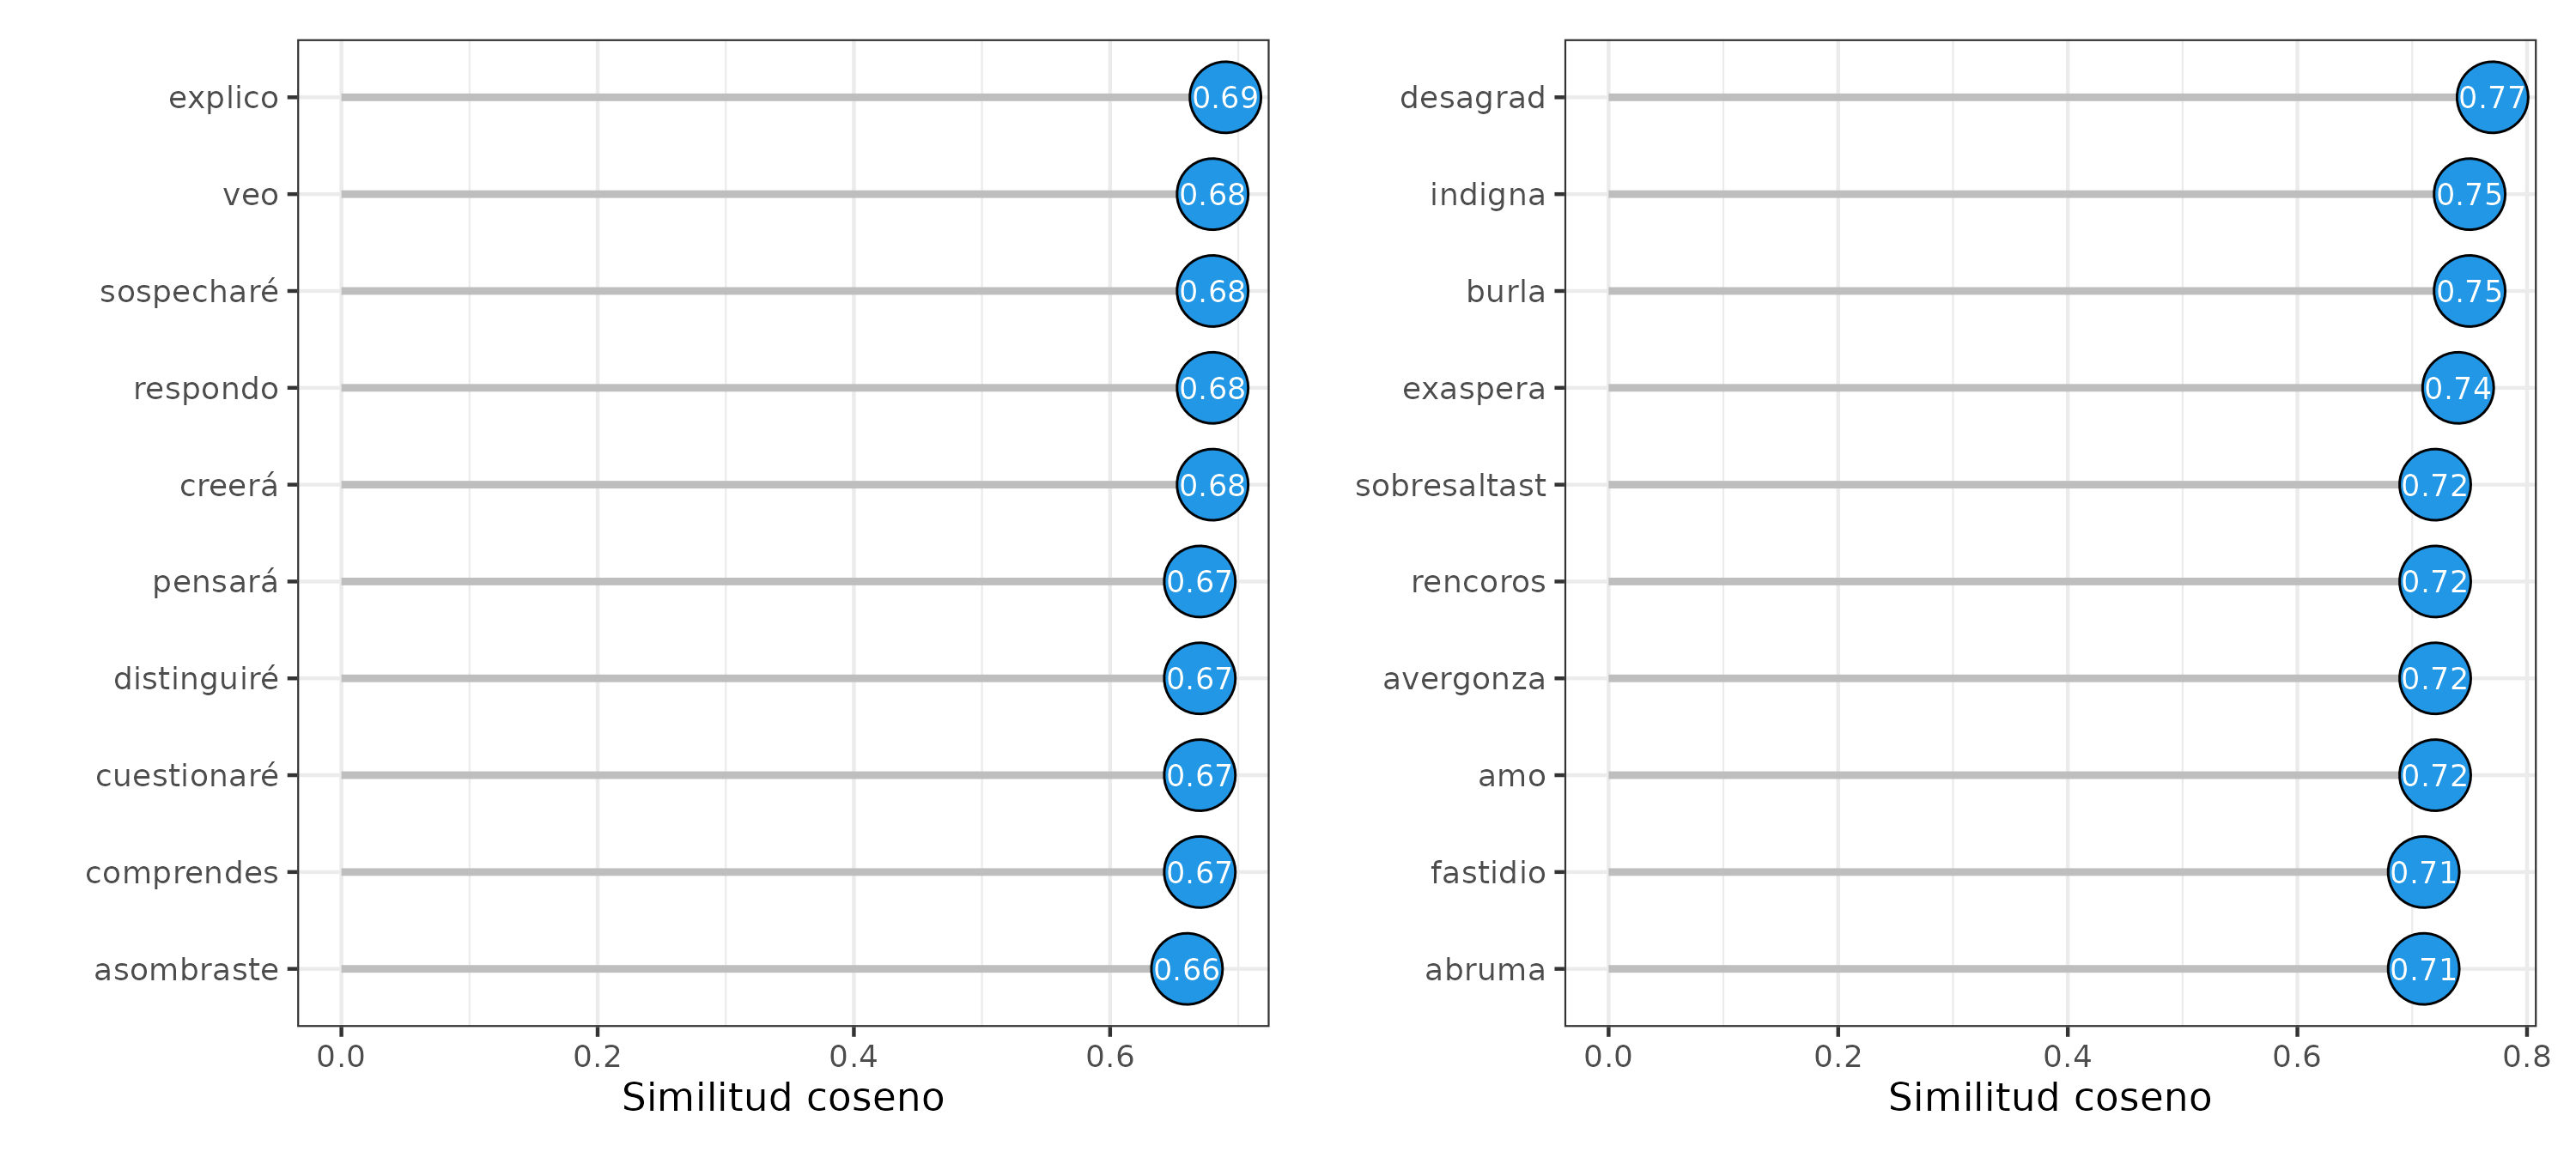
\includegraphics[width = 0.7 \textwidth]{cuadros_tesis/plot_important_words.png}
\normalsize
\end{figure}

Con el objetivo de validar que los vectores efectivamente estén midiendo
afectividad y cognición, es importante observar cuáles son las palabras
del corpus que más se acercan a cada una de las polaridades. Para ello,
se calculó la similitud coseno entre cada una de las
193.205\footnote{Este número corresponde al total de palabras luego de haber aplicado un procedimiento de tokenización, mediante el cual se eliminan *stoptwords* y se seleccionan solo los adjectivos, sustantivos y verbos}
palabras del corpus que no están dentro del diccionario y los vectores
que representan a los polos cognitivo y afectivo. Las figuras
\ref{fig:nube_afectiva} \ref{fig:nube_cognitiva} muestran a través de su
tamaño cuán cerca se encuentra una palabra de cada una de las
polaridades. Se observa que, efectivamente, los vectores construidos
para cada una de las polaridades dan cuenta de afectividad y cognición,
ya que mientras en el panel izquierdo (polaridad afectiva) palabras como
\emph{rencoroso}, \emph{atormentado} y \emph{enfado} muestran una
presencia importante, en el panel derecho resaltan verbos como
\emph{decir}, \emph{demostrar} y \emph{preguntar}.

Cabe mencionar que las palabras del polo afectivo presentan un sesgo
hacia emociones tradicionalmente consideradas como negativas. El motivo
de ello es que el diccionario utilizado tiene un sesgo hacia palabras de
este tipo, lo que implica que la construcción del vector de afectividad
esté sesgado hacia ese tipo de emociones, cuestión que debe tenerse en
consideración al momento de analizar los resultados. Con el objeto de
descartar que el polo afectivo esté capturando únicamente emociones
negativas, se llevaron a cabo algunas pruebas con palabras usualmente
consideradas positivas como \emph{amor}, \emph{alegría} o \emph{risa}.
Este ejercicio arrojó como resultado una asociación más fuerte con el
vector emotivo que con el cognitivo, lo que da cuenta de que si bien
existe un sesgo hacia emociones negativas, el instrumento es capaz de
dar cuenta también de emociones positivas.

\begin{figure}[H]
     \caption{Nubes de palabras }
     \centering
     \begin{subfigure}[b]{0.4\textwidth}
         \centering
         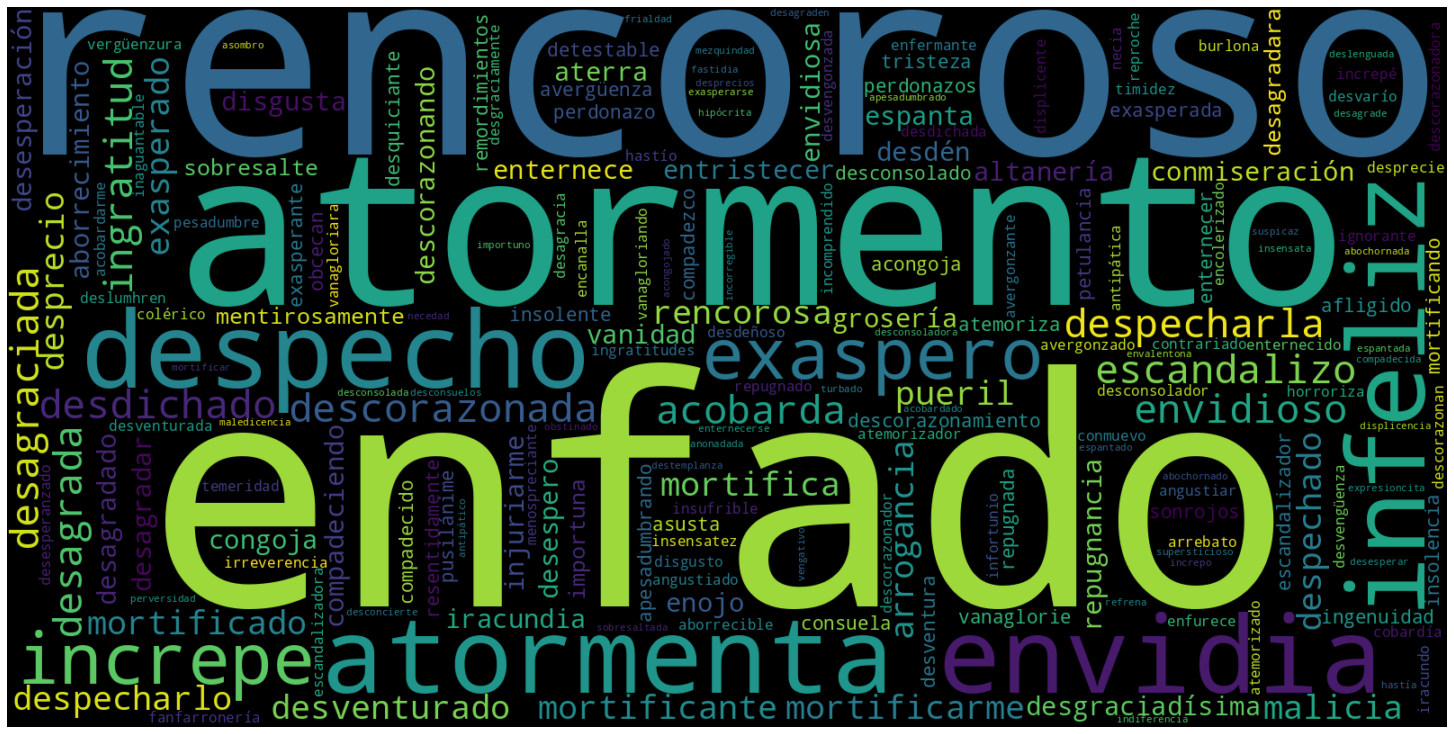
\includegraphics[width=\textwidth]{cuadros_tesis/wordcloud_affective.png}
         \caption{Polo afectivo}
         \label{fig:nube_afectiva}
     \end{subfigure}
     \begin{subfigure}[b]{0.4\textwidth}
         \centering
         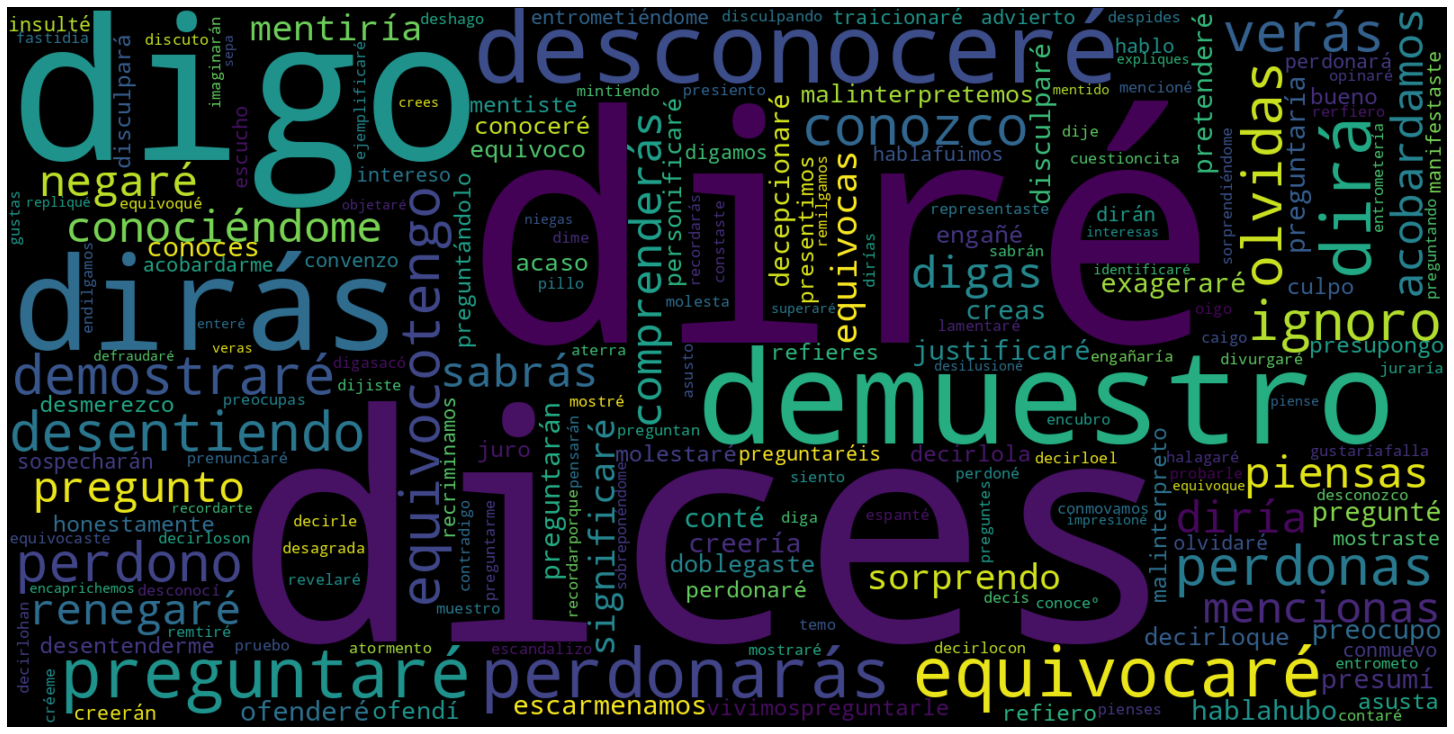
\includegraphics[width=\textwidth]{cuadros_tesis/wordcloud_cognitive.png}
         \caption{Polo cognitivo}
         \label{fig:nube_cognitiva}
     \end{subfigure}
     \label{fig:nubes}
     \caption*{\footnotesize{\textit{Nota:} Cada nube contiene las 200 palabras con mayor similitud coseno respecto a los vectores cognitivo y afectivo. El tamaño de las palabras se pondera de acuerdo al valor de la similitud coseno.}}
\end{figure}

\hypertarget{identificaciuxf3n-de-la-polaridad}{%
\subsection{Identificación de la
polaridad}\label{identificaciuxf3n-de-la-polaridad}}

\hypertarget{identificaciuxf3n-de-tuxf3picos}{%
\subsection{Identificación de
tópicos}\label{identificaciuxf3n-de-tuxf3picos}}

\hypertarget{polarizaciuxf3n-poluxedtica}{%
\subsection{Polarización política}\label{polarizaciuxf3n-poluxedtica}}

\hypertarget{resultados}{%
\section{Resultados}\label{resultados}}

\hypertarget{estaduxedstica-descriptiva-polos-y-tuxf3picos}{%
\subsection{Estadística descriptiva polos y
tópicos}\label{estaduxedstica-descriptiva-polos-y-tuxf3picos}}

\hypertarget{regresiuxf3n}{%
\subsection{Regresión}\label{regresiuxf3n}}

\hypertarget{conclusiones}{%
\section{Conclusiones}\label{conclusiones}}

Mis grandes conclusiones

\newpage

\hypertarget{referencias}{%
\section*{Referencias}\label{referencias}}
\addcontentsline{toc}{section}{Referencias}

\hypertarget{refs}{}
\begin{CSLReferences}{1}{0}
\leavevmode\vadjust pre{\hypertarget{ref-fasttext}{}}%
Bojanowski, Piotr, Edouard Grave, Armand Joulin, y Tomás Mikolov. 2016.
{«Enriching Word Vectors with Subword Information»}. \emph{CoRR}
abs/1607.04606. \url{http://arxiv.org/abs/1607.04606}.

\leavevmode\vadjust pre{\hypertarget{ref-aggarwal}{}}%
Charu C., Aggarwal. 2018. \emph{Neural Networks and Deep Learning. A
Textbook}. Springer Cham.
https://doi.org/\url{https://doi.org/10.1007/978-3-319-73004-2}.

\leavevmode\vadjust pre{\hypertarget{ref-paper_central}{}}%
Gennaro, Gloria, y Elliott Ash. 2021. {«{Emotion and Reason in Political
Language}»}. \emph{The Economic Journal} 132 (643): 1037-59.
\url{https://doi.org/10.1093/ej/ueab104}.

\leavevmode\vadjust pre{\hypertarget{ref-linguistic_dictionary}{}}%
Pennebaker, J. W., R. L. Boyd, K. Jordan, y K. Blackburn. 2015.
\emph{The development and psychometric properties of LIWC2015}. Austin,
TX: University of Texas at Austin.
\url{https://www.liwc.app/static/documents/LIWC2015\%20Manual\%20-\%20Development\%20and\%20Psychometrics.pdf}.

\leavevmode\vadjust pre{\hypertarget{ref-word_embeddings}{}}%
Perez, Jorge, y José Cañete. 2019. {«Spanish Word Embeddings»}.
\url{https://github.com/dccuchile/spanish-word-embeddings}.

\leavevmode\vadjust pre{\hypertarget{ref-intro_deep_learning}{}}%
Skansi, Sandro. 2018. \emph{Introduction to Deep Learning. From Logical
Calculus to Artificial Intelligence}. Springer Cham.
https://doi.org/\url{https://doi.org/10.1007/978-3-319-73004-2}.

\end{CSLReferences}

\end{document}
